\documentclass[journal,10pt,twocolumn]{article}
\usepackage{graphicx}
\graphicspath{{./Figures/}}
\usepackage[margin=0.5in]{geometry}
\usepackage[cmex10]{amsmath}
\usepackage{amssymb}
\usepackage{array}
\usepackage{booktabs}
\title{\textbf{Circle Assignment}}
\author{Bole Manideep}
\date{September 2022}


\providecommand{\pr}[1]{\ensuremath{\Pr\left(#1\right)}}
\providecommand{\qfunc}[1]{\ensuremath{Q\left(#1\right)}}
\providecommand{\sbrak}[1]{\ensuremath{{}\left[#1\right]}}
\providecommand{\lsbrak}[1]{\ensuremath{{}\left[#1\right.}}
\providecommand{\rsbrak}[1]{\ensuremath{{}\left.#1\right]}}
\providecommand{\brak}[1]{\ensuremath{\left(#1\right)}}
\providecommand{\lbrak}[1]{\ensuremath{\left(#1\right.}}
\providecommand{\rbrak}[1]{\ensuremath{\left.#1\right)}}
\providecommand{\cbrak}[1]{\ensuremath{\left\{#1\right\}}}
\providecommand{\lcbrak}[1]{\ensuremath{\left\{#1\right.}}
\providecommand{\rcbrak}[1]{\ensuremath{\left.#1\right\}}}
\providecommand{\norm}[1]{\left\lVert#1\right\rVert}
\providecommand{\abs}[1]{\left\vert#1\right\vert}
\let\vec\mathbf
\newcommand{\myvec}[1]{\ensuremath{\begin{pmatrix}#1\end{pmatrix}}}
\newcommand{\mydet}[1]{\ensuremath{\begin{vmatrix}#1\end{vmatrix}}}
\providecommand{\brak}[1]{\ensuremath{\left(#1\right)}}

\begin{document}

\maketitle
\paragraph{\large{\textit{Problem Statement} - Draw a circle of radius 3 cm. Take two points P and Q on one of its extended diameter each at a distance of 7 cm from its centre. Draw tangents to the circle from these two points P and Q.}}
\begin{enumerate}
	\item \large Radius of circle OA = OB = 3cm
	\item \large Distance from center to points OP = OQ = 7cm
\end{enumerate}

\begin{figure}[h]
\centering
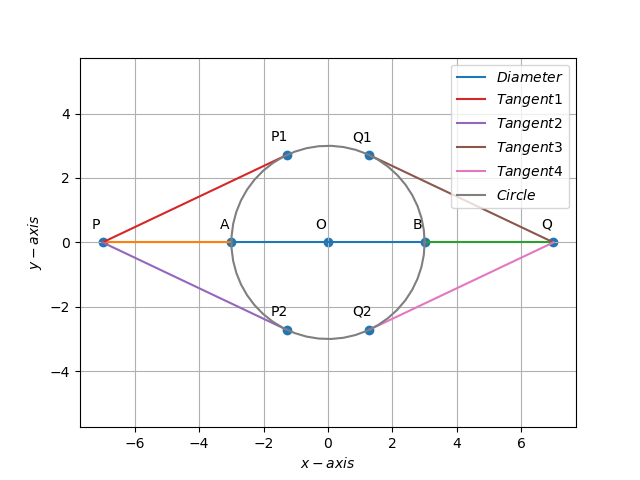
\includegraphics[width=1\columnwidth]{Question.png}
\caption{Circle with center O and points P \& Q}
\label{fig:Circle}
\end{figure}

\section*{Solution}

\raggedright \large{Consider the circle of radius 3cm whose center is at origin and points P \& Q each at a distance of 7cm from the center. \\
Two tangents can be drawn from point P on to the circle and let the point of contacts be P1 and P2, and other two tangents can be drawn from point Q on to the circle and let the point of contacts be Q1 and Q2} \\ \vspace{2mm}

\large{The point of intersection of line}
\begin{align}
L: \quad \vec{x} = \vec{q} + \mu \vec{m} \quad \mu \in \mathbb{R}\end{align}
\large{with the conic section}
\begin{align}
\vec{x}^{\top}\vec{V}\vec{x}+2\vec{u}^{\top}\vec{x}+f=0
\end{align}
\large{is given by}
\begin{align}
\vec{x}_i = \vec{q} + \mu_i \vec{m}
\end{align}
\large{where}
\begin{multline}
\mu_i = \frac{1}{\vec{m}^{\top}\vec{V}\vec{m}}
\lbrak{-\vec{m}^{\top}\brak{\vec{V}\vec{q}+\vec{u}}}
\\
\pm{\small\rbrak{\sqrt{\sbrak{\vec{m}^{\top}\brak{\vec{V}\vec{q} \vec{u}}}^2-\brak{\vec{q}^{\top}\vec{V}\vec{q} + 2\vec{u}^{\top}\vec{q} +f}\brak{\vec{m}^{\top}\vec{V}\vec{m}}}}}
\end{multline}
\large{If the line L touches the conic at exactly one point $\vec{q}$,}
\begin{align}
\vec{m}^{\top}\brak{\vec{V}\vec{q}+\vec{u}} = 0
\end{align}
\large{In this case, the conic intercept has exactly one root.Hence,}
\begin{align}
\sbrak{\vec{m}^{\top}\brak{\vec{V}\vec{q}+\vec{u}}}^2 -\brak{\vec{m}^{\top}\vec{V}\vec{m}}\brak{\vec{q}^{\top}\vec{V}\vec{q} + 2\vec{u}^{\top}\vec{q} +f} = 0                                                                                             
\end{align}\vspace{0.5cm}
\large{So, the equation of conic  $x^2 + y^2 = 9$ can be written in the form of eq (2) as,}
\begin{align}
\vec{x}^{\top}\myvec{1&0\\0&1}\vec{x}+2\myvec{0&0}\vec{x}+9=0
\end{align}
\large{Let us conisder the direction vector of $\vec{L}$ as m,}
\begin{align}
\vec{m}=\myvec{1 \\ \lambda}
\end{align}
\large{and $\vec{q}$ be the point P,}
\begin{align}
\vec{q}=\myvec{-7 \\ 0}
\end{align}

\large{Substituting (7),(8) and (9) in eq (6), we get}
\begin{align*}
\sbrak{\vec{m}^{\top}\brak{\vec{I}\vec{q}}}^2 - \brak{\vec{m}^{\top}\vec{I}\vec{m}}\brak{\vec{q}^{\top}\vec{I}\vec{q}+(-9)} =0
\end{align*}
\begin{multline}
\sbrak{\myvec{1 & \lambda}\myvec{-7 \\ 0}}^2 \\ - \brak{\myvec{1 & \lambda}\myvec{1 \\ \lambda}}\brak{\myvec{-7 & 0}\myvec{-7 \\ 0}-9} = 0
\end{multline}
\begin{gather*}
\brak{-7}^2-\brak{1+\lambda^2}\brak{49-9} = 0 \\
49 - \brak{1+\lambda^2}\brak{40} = 0 \\
\brak{1+\lambda^2}\brak{40} = 49 \\
1+\lambda^2 = \frac{49}{40} \\
\lambda^2 = \frac{9}{40} \\
\lambda = \pm \frac{3}{\sqrt{40}}
\end{gather*}
\begin{equation}
\lambda = \pm 0.4743
\end{equation}
That is,
\begin{equation}
\vec{m} = \myvec{1 \\ \pm 0.4743}
\end{equation}
From (4) and (6)
\begin{equation}
\mu_i = \frac{1}{\vec{m}^{\top}\vec{V}\vec{m}}
\lbrak{-\vec{m}^{\top}\brak{\vec{V}\vec{q}+\vec{u}}}
\end{equation}
\begin{gather*}
\mu_i = \frac{1}{\myvec{1 & \frac{3}{\sqrt{40}}}\vec{I}\myvec{1 \\ \frac{3}{\sqrt{40}}}}\lbrak{-\myvec{1 & \sqrt{40}}\brak{\vec{I}\myvec{-7 \\ 0}}} \\ \vspace{4mm}
\mu_i = \frac{1}{1+\frac{9}{40}}\brak{-7+0} \\
\mu_i = \frac{-7}{\brak{\frac{49}{40}}} \\
\mu_i = \frac{40}{7}
\end{gather*}
\begin{equation}
\mu_i = 5.714
\end{equation}
Now (3) becomes,
\begin{equation}
\myvec{x \\ y} = \myvec{-7 \\ 0}+5.714*\myvec{1 \\ \pm 0.4743}
\end{equation}
\begin{equation}
\myvec{x \\ y} = \myvec{-7 \\ 0}+\myvec{5.714 \\ \pm 2.710}
\end{equation}
\begin{equation}
\implies \hspace{4mm} \myvec{x \\ y} = \myvec{-1.285 \\ 2.710} \hspace{2mm} or \hspace{2mm} \myvec{x \\ y} = \myvec{-1.285 \\ -2.710}
\end{equation}
Therefore,
\begin{align*}
\vec{P_1} = \myvec{-1.285 \\ 2.710} \\
\vec{P_2} = \myvec{-1.285 \\ -2.710}
\end{align*}
In the similar way, points of contact from the other point Q that are $Q_1 \hspace{2mm} \& \hspace{2mm} Q_2$ can be
\begin{align*}
\vec{Q_1} = \myvec{1.285 \\ 2.710} \\
\vec{Q_2} = \myvec{1.285 \\ -2.710}
\end{align*}


\section*{Construction}
\raggedright A Circle with center O and radius 3cm is constructed unsing python,with the parameters that are mentioned in the table below.
\vspace{5mm}
\begin{center}
    \setlength{\arrayrulewidth}{0.1mm}
	\setlength{\tabcolsep}{5pt}
	\renewcommand{\arraystretch}{1.5}
\begin{tabular}{|c|c|c|}
	\hline 
    \textbf{Symbol} & \textbf{Value} & \textbf{Description}\\ 		\hline
    r & 3 & Radius \\ \hline
    d & 7 & distance from O to P \& Q \\ \hline
    $\vec{O}$ & $\myvec{0 \\ 0}$ & Center \\ \hline
    $\vec{e_1}$ & $\myvec{1 \\ 0}$ & Unit Vector \\ \hline
    $\vec{P}$ & -d$\ast\vec{e1}$ & Point P \\ \hline
    $\vec{Q}$ & d$\ast\vec{e1}$ & Point Q \\ \hline
    $\theta$ & $\angle P_1OP$ & Angle $P_1PO$ \\ \hline
    $\vec{P_1}$ & $r\myvec{cos(\pi-\theta) \\ sin(\pi-\theta)}$ & 		Point of contact P1 \\ \hline
    $\vec{P_2}$ & $r\myvec{cos(\pi-\theta) \\ -sin(\pi-\theta)}$ & 		Point of contact P2 \\ \hline
    $\vec{Q_1}$ & $r\myvec{cos\theta \\ sin\theta}$ & Point of contact Q1 \\ \hline
    $\vec{Q_2}$ & $r\myvec{cos\theta \\ -sin\theta}$ & Point of contact Q2 \\ \hline
\end{tabular}\\ \vspace{2mm}
Table 1: Parameter's Table
\end{center}
 






\end{document}
